% Created 2019-03-07 Thu 12:04
% Intended LaTeX compiler: pdflatex
\documentclass[11pt]{article}
\usepackage[utf8]{inputenc}
\usepackage[T1]{fontenc}
\usepackage{graphicx}
\usepackage{grffile}
\usepackage{longtable}
\usepackage{wrapfig}
\usepackage{rotating}
\usepackage[normalem]{ulem}
\usepackage{amsmath}
\usepackage{textcomp}
\usepackage{amssymb}
\usepackage{capt-of}
\usepackage{hyperref}
\author{Francisco Viramontes}
\date{\today}
\title{}
\hypersetup{
 pdfauthor={Francisco Viramontes},
 pdftitle={},
 pdfkeywords={},
 pdfsubject={},
 pdfcreator={Emacs 26.1 (Org mode 9.2.1)}, 
 pdflang={English}}
\begin{document}

\tableofcontents

\section{Project deps}
\label{sec:org5cc2e06}

\begin{verbatim}
{:deps 
 {fundingcircle/jackdaw {:mvn/version "0.6.0"}
  ;;org.apache.kafka/kafka-streams {:mvn/version "2.1.0"}
  ;;org.apache.kafka/kafka-streams-test-utils {:mvn/version "2.1.0"}
  org.clojure/clojure {:mvn/version "1.10.0"}
  org.clojure/tools.logging {:mvn/version "0.4.1"}}

 :mvn/repos
 {"confluent" {:url "https://packages.confluent.io/maven/"}}

 :paths
 ["src" "test" "dev"]

 :aliases
 {:test {:extra-deps {com.cognitect/test-runner
                      {:git/url "https://github.com/cognitect-labs/test-runner.git"
                       :sha "209b64504cb3bd3b99ecfec7937b358a879f55c1"}}
         :main-opts ["-m" "cognitect.test-runner"]}}}

\end{verbatim}

\section{Confluent tools}
\label{sec:org32b4ef8}
\subsection{Manage Confluent tools on the REPL}
\label{sec:org178699e}
\begin{verbatim}
(ns confluent
  "Functions to start and stop ZooKeeper and Kafka.
  These functions require the Confluent Platform CLI which can be
  obtained from `https://www.confluent.io/download/`.
  WARNING: Quitting the REPL will not stop ZooKeeper and Kafka. Before
  exiting, you must invoke `confluent/stop`. Otherwise, run `confluent
  destroy` from the command line."
  (:require [clojure.string :as str]
            [clojure.java.shell :refer [sh]]))

(defn not-up
  "Takes `service` and returns true if the service is down"
  [service]
  (->> (:out (sh "confluent" "status"))
       str/split-lines
       (keep (fn [x] (re-find (re-pattern (str service " is.*")) x)))
       first
       (re-find #"DOWN")
       boolean))

(defn stop
  "Starts ZooKeeper and Kafka."
  []
  (sh "confluent" "destroy")
  (println "schema-registry is down")
  (println "kafka is down")
  (println "zookeeper is down"))

(defn start
  "Starts ZooKeeper and Kafka."
  []
  (with-out-str (stop))
  (doseq [s ["zookeeper" "kafka" "schema-registry"]]
    (do (while (not-up s)
          (sh "confluent" "start" s)
          (Thread/sleep 1000))
        (println s "is up"))))

(defn reset
  "Stops and starts ZooKeeper and Kafka."
  []
  (stop)
  (start))
\end{verbatim}
\subsection{Start confluent platform}
\label{sec:org67d4751}
\begin{verbatim}
(confluent/start)
\end{verbatim}
\section{Helpful helpers}
\label{sec:org5a7b76a}

\begin{verbatim}
(ns user
  "your lovely home"
  (:require [clojure.java.shell :refer [sh]]
            [jackdaw.client :as jc]
            [jackdaw.client.log :as jcl]
            [jackdaw.admin :as ja]
            [jackdaw.serdes.edn :as jse]
            [jackdaw.streams :as j]
            [confluent])
  (:import org.apache.kafka.common.serialization.Serdes))

;;; ------------------------------------------------------------
;;;
;;; Configure topics
;;;
(defn topic-config
  "Takes a topic name and (optionally) key and value serdes and a
  partition count, and returns a topic configuration map, which may be
  used to create a topic or produce/consume records."
  ([topic-name]
   (topic-config topic-name (jse/serde)))

  ([topic-name value-serde]
   (topic-config topic-name (jse/serde) value-serde))

  ([topic-name key-serde value-serde]
   (topic-config topic-name 1 key-serde value-serde))

  ([topic-name partition-count key-serde value-serde]
   {:topic-name topic-name
    :partition-count partition-count
    :replication-factor 1
    :topic-config {}
    :key-serde key-serde
    :value-serde value-serde}))

;;; ------------------------------------------------------------
;;;
;;; Create, delete and list topics
;;;
(defn kafka-admin-client-config
  []
  {"bootstrap.servers" "localhost:9092"})

(defn create-topics
  "Takes a list of topics and creates these using the names given."
  [topic-config-list]
  (with-open [client (ja/->AdminClient (kafka-admin-client-config))]
    (ja/create-topics! client topic-config-list)))

(defn re-delete-topics
  "Takes an instance of java.util.regex.Pattern and deletes any Kafka
  topics that match."
  [re]
  (with-open [client (ja/->AdminClient (kafka-admin-client-config))]
    (let [topics-to-delete (->> (ja/list-topics client)
                                (filter #(re-find re (:topic-name %))))]
      (ja/delete-topics! client topics-to-delete))))

(defn create-topic
  "Takes a single topic config and creates a Kafka topic."
  [topic-config]
  (create-topics [topic-config]))

(defn list-topics
  "Returns a list of Kafka topics."
  []
  (with-open [client (ja/->AdminClient (kafka-admin-client-config))]
    (ja/list-topics client)))

(defn topic-exists?
  "Takes a topic name and returns true if the topic exists."
  [topic-config]
  (with-open [client (ja/->AdminClient (kafka-admin-client-config))]
    (ja/topic-exists? client topic-config)))

;;; ------------------------------------------------------------
;;;
;;; Produce and consume records
;;;

(defn kafka-producer-config
  []
  {"bootstrap.servers" "localhost:9092"})

(defn kafka-consumer-config
  [group-id]
  {"bootstrap.servers" "localhost:9092"
   "group.id" group-id
   "auto.offset.reset" "earliest"
   "enable.auto.commit" "false"})

(defn publish
  "Takes a topic config and record value, and (optionally) a key and
  parition number, and produces to a Kafka topic."
  ([topic-config value]
   (with-open [client (jc/producer (kafka-producer-config) topic-config)]
     @(jc/produce! client topic-config value))
   nil)

  ([topic-config key value]
   (with-open [client (jc/producer (kafka-producer-config) topic-config)]
     @(jc/produce! client topic-config key value))
   nil)

  ([topic-config partition key value]
   (with-open [client (jc/producer (kafka-producer-config) topic-config)]
     @(jc/produce! client topic-config partition key value))
   nil))

(defn get-records
  "Takes a topic config, consumes from a Kafka topic, and returns a
  seq of maps."
  ([topic-config]
   (get-records topic-config 200))

  ([topic-config polling-interval-ms]
   (let [client-config (kafka-consumer-config
                        (str (java.util.UUID/randomUUID)))]
     (with-open [client (jc/subscribed-consumer client-config
                                                [topic-config])]
       (doall (jcl/log client 100 seq))))))

(defn get-keyvals
  "Takes a topic config, consumes from a Kafka topic, and returns a
  seq of key-value pairs."
  ([topic-config]
   (get-keyvals topic-config 20))

  ([topic-config polling-interval-ms]
   (map (juxt :key :value) (get-records topic-config polling-interval-ms))))

;;; ------------------------------------------------------------
;;;
;;; System
;;;

(def system nil)
\end{verbatim}

\section{Simple pipe topology example}
\label{sec:orgb7cf5a4}
\subsection{Overview}
\label{sec:orgefb425f}
\begin{center}
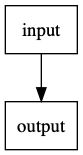
\includegraphics[width=.9\linewidth]{pipe.png}
\end{center}

\subsection{Define topology}
\label{sec:org38e841e}
\begin{verbatim}
(ns pipe
  "This tutorial contains a simple stream processing application using
  Jackdaw and Kafka Streams.
  Pipe reads from a Kafka topic called `input`, logs the key and
  value, and writes these to a Kafka topic called `output`."
  (:gen-class)
  (:require [clojure.string :as str]
            [clojure.tools.logging :refer [info]]
            [jackdaw.streams :as j]
            [jackdaw.serdes.edn :as jse])
  (:import [org.apache.kafka.common.serialization Serdes]))

(defn topic-config
  "Takes a topic name and returns a topic configuration map, which may
  be used to create a topic or produce/consume records."
  [topic-name]
  {:topic-name topic-name
   :partition-count 1
   :replication-factor 1
   :key-serde (jse/serde)
   :value-serde (jse/serde)})

(defn app-config
  "Returns the application config."
  []
  {"application.id" "word-count"
   "bootstrap.servers" "localhost:9092"
   "cache.max.bytes.buffering" "0"})

(defn build-topology
  "Reads from a Kafka topic called `input`, logs the key and value,
  and writes these to a Kafka topic called `output`. Returns a
  topology builder."
  [builder]
  (-> (j/kstream builder (topic-config "input"))
      (j/peek (fn [[k v]]
                (info (str {:key k :value v}))))
      (j/to (topic-config "output")))
  builder)

(defn start-app
  "Starts the stream processing application."
  [app-config]
  (let [builder (j/streams-builder)
        topology (build-topology builder)
        app (j/kafka-streams topology app-config)]
    (j/start app)
    (info "pipe is up")
    app))

(defn stop-app
  "Stops the stream processing application."
  [app]
  (j/close app)
  (info "pipe is down"))

(defn -main
  [& _]
  (start-app (app-config)))
\end{verbatim}

\subsection{Define topology start stop}
\label{sec:org04cc845}
\begin{verbatim}
(require '[pipe])

(defn stop-pipe
  "Stops the app, and deletes topics and internal state."
  []
  (when (and system (:pipe-app system))
    (pipe/stop-app (:pipe-app system)))
  (re-delete-topics #"(input|output)")
  (alter-var-root #'system merge {:pipe-app nil}))

(defn start-pipe
  "Creates topics, and starts the app."
  []
  (create-topics (map pipe/topic-config ["input" "output"]))
  (alter-var-root #'system merge {:pipe-app (pipe/start-app (pipe/app-config))}))
\end{verbatim}

\subsection{Start/reset topology state}
\label{sec:orgd2c2b7a}
\begin{verbatim}
(stop-pipe)

(Thread/sleep 1000)

(start-pipe)
\end{verbatim}

\subsection{List topics}
\label{sec:orgb388eb7}
\begin{verbatim}
(list-topics)
\end{verbatim}
\subsection{List publish input}
\label{sec:orge4f9847}
\begin{verbatim}
(publish (topic-config "input") "mundo")
\end{verbatim}
\subsection{Read from the output}
\label{sec:orgd528830}
\begin{verbatim}
(get-keyvals (topic-config "output"))
\end{verbatim}
\section{The flex app}
\label{sec:org74afadb}
\subsection{Overview}
\label{sec:org53c7bf1}
\begin{center}
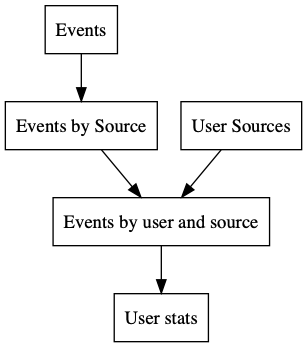
\includegraphics[width=.9\linewidth]{flex.png}
\end{center}

\subsection{Define topology}
\label{sec:orgf7f5103}
\begin{verbatim}
(ns flex
  ""
  (:gen-class)
  (:require [clojure.string :as str]
            [clojure.tools.logging :refer [info]]
            [jackdaw.streams :as j]
            [jackdaw.serdes.edn :as jse])
  (:import [org.apache.kafka.common.serialization Serdes]))

(defn topic-config
  "Takes a topic name and returns a topic configuration map, which may
  be used to create a topic or produce/consume records."
  [topic-name]
  {:topic-name topic-name
   :partition-count 1
   :replication-factor 1
   :key-serde (jse/serde)
   :value-serde (jse/serde)})

(defn app-config
  "Returns the application config."
  []
  {"application.id" "flex-app"
   "bootstrap.servers" "localhost:9092"
   "cache.max.bytes.buffering" "0"})

(defn build-topology
  ""
  [builder]
  (let [event-stream (j/kstream builder (topic-config "events"))
        user-sources-table (j/ktable builder (topic-config "user-sources"))
        events-by-source (-> event-stream
                             (j/map (fn [[_ v]]
                                      [(:source-id v) v]))
                             (j/through (topic-config "events-by-source")))
        events-by-user-and-source (-> events-by-source
                                      (j/left-join user-sources-table
                                                   (fn [event user-source]
                                                     (merge event user-source))
                                                   (topic-config "")
                                                   (topic-config ""))
                                      (j/map (fn [[_ v]]
                                               [[(:user-id v) (:source-id v)] v]))
                                      (j/through (topic-config "events-by-user-and-source")))]
    (-> events-by-user-and-source
        (j/group-by-key (topic-config ""))
        (j/aggregate (constantly {:count 0 :sum 0})
                     (fn [acc [k v]]
                       (-> acc
                           (update :count inc)
                           (update :sum #(+ % (:value v)))
                           (merge (select-keys v [:name :user-id]))))
                     (topic-config "user-stats"))
        (j/to-kstream)
        (j/to (topic-config "user-stats")))
    builder))

(defn start-app
  "Starts the stream processing application."
  [app-config]
  (let [builder (j/streams-builder)
        topology (build-topology builder)
        app (j/kafka-streams topology app-config)]
    (j/start app)
    (info "flex is up")
    app))

(defn stop-app
  "Stops the stream processing application."
  [app]
  (j/close app)
  (info "flex is down"))

(defn -main
  [& _]
  (start-app (app-config)))
\end{verbatim}

\subsection{Define topology start stop}
\label{sec:orgfc37134}
\begin{verbatim}
(require '[flex])

(defn stop-flex
  "Stops the app, and deletes topics and internal state."
  []
  (when (and system (:flex-app system))
    (flex/stop-app (:flex-app system))
    (.cleanUp (:flex-app system)) ;; clears internal state topics
    )
  (re-delete-topics #"(events|events-by-source|events-by-user-and-source|user-sources|user-stats)")
  (alter-var-root #'system merge {:flex-app nil}))

(defn start-flex
  "Creates topics, and starts the app."
  []
  (create-topics (map flex/topic-config ["events" "events-by-source" "events-by-user-and-source" "user-sources" "user-stats"]))
  (alter-var-root #'system merge {:flex-app (flex/start-app (flex/app-config))}))
\end{verbatim}

\subsection{Start/reset topology state}
\label{sec:orgabd90e8}
\begin{verbatim}
(stop-flex)

(Thread/sleep 1000)

(start-flex)
\end{verbatim}

\subsection{List topics}
\label{sec:org6d9a8e9}
\begin{verbatim}
(list-topics)
\end{verbatim}

\subsection{List publish input}
\label{sec:org51993a0}
\begin{verbatim}
(def user-1 (java.util.UUID/randomUUID))

(def source-1 (java.util.UUID/randomUUID))

(def source-2 (java.util.UUID/randomUUID))

(def user-2 (java.util.UUID/randomUUID))

(def source-3 (java.util.UUID/randomUUID))


(publish (topic-config "user-sources")
         source-1
         {:name "step counter"
          :user-id user-1})

(publish (topic-config "user-sources")
         source-2
         {:name "pushup counter"
          :user-id user-1})

(publish (topic-config "user-sources")
         source-3
         {:name "step counter"
          :user-id user-2})

(publish (topic-config "events")
         {:event-id (java.util.UUID/randomUUID)
          :source-id source-1
          :value 1
          :timestamp (System/currentTimeMillis)})

(publish (topic-config "events")
         {:event-id (java.util.UUID/randomUUID)
          :source-id source-2
          :value 2
          :timestamp (System/currentTimeMillis)})

(publish (topic-config "events")
         {:event-id (java.util.UUID/randomUUID)
          :source-id source-3
          :value 100
          :timestamp (System/currentTimeMillis)})

(publish (topic-config "events")
         {:event-id (java.util.UUID/randomUUID)
          :source-id source-2
          :value 100
          :timestamp (System/currentTimeMillis)})

\end{verbatim}

\subsection{Read from the output}
\label{sec:org15da23f}
\begin{verbatim}
(get-keyvals (topic-config "events"))

(get-keyvals (topic-config "user-sources"))

(get-keyvals (topic-config "events-by-source"))

(get-keyvals (topic-config "events-by-user-and-source"))

(get-keyvals (topic-config "user-stats"))

(get-keyvals (topic-config "flex-app-user-stats-changelog"))

\end{verbatim}
\end{document}
